%==============================================================================
%  Project report: Bayesian Networks and Markov Models in Action AIDAMS Y4 2026
%==============================================================================
\documentclass[12pt]{article}

\usepackage[utf8]{inputenc}
\usepackage[T1]{fontenc}
\usepackage[english]{babel}
\usepackage{amsmath,amssymb,amsfonts}
\usepackage{graphicx}
\usepackage{booktabs}
\usepackage{xcolor}
\usepackage[ruled,vlined]{algorithm2e}
\usepackage[colorlinks=true,linkcolor=black,citecolor=blue,urlcolor=blue]{hyperref}

\usepackage{fancyhdr}
\pagestyle{fancy}

\usepackage[left=2.5cm,right=2.5cm,top=2.5cm,bottom=2.5cm]{geometry}
\setlength{\parskip}{6pt}

\usepackage[capitalise,noabbrev]{cleveref}

\newcommand{\guide}[1]{\textit{\textcolor{gray}{#1}}}

% Notation used in the course 
\newcommand{\E}{\mathbb{E}}
\newcommand{\by}{\mathbf{y}}
\newcommand{\given}{\,\vert\,}

% Author-year citations in brackets + the Bayesian network diagram
\usepackage{natbib}
\usepackage{tikz}
\usetikzlibrary{positioning}
\usepackage{float}   % [H]: keep appendix figures right under section title

\renewcommand{\headrulewidth}{0pt}

\pagestyle{fancy}
\fancyhead{}
\fancyfoot{}
\fancyfoot[L]{Bayesian Networks and Markov Models in Action}
\fancyfoot[R]{\thepage}
\fancyhead{}


\begin{document}

%--------------------------------------------------------------------------
%  Title and authors
%--------------------------------------------------------------------------

\begin{center}
{\Large\sc Engaged or browsing?}\\[0.6em]
{\large\sc A Bayesian hidden Markov model of music skips}
\bigskip

Aliénor Sabourdin, Anastasia Bouev-Dombre \& Elise Deyris
\bigskip

{\it
BSc in Artificial Intelligence, Data \& Management Sciences, CentraleSupélec -- Université Paris-Saclay \& ESSEC, France
}
\end{center}

\bigskip

%--------------------------------------------------------------------------
%  Abstract
%--------------------------------------------------------------------------
{\bf Abstract.} When a listener skips a track, is it because of the track itself, or because of the listener's mood? We study 5{,}375 listening sessions built from Yambda, a public music-streaming data set, and ask whether a hidden mood, engaged or browsing, can be inferred from skips alone, and whether it can change within a listening session. We compare three Bayesian models of growing complexity: one skip rate for all tracks (Beta--Bernoulli), one hidden type per session that never changes (a latent-class model), and moods that switch from track to track (a hidden Markov model). We find the posterior mode with EM and the full posterior with importance sampling, using a Student-$t$ proposal on the log-odds scale. Both methods are validated on simulated data, where the true values fall inside the posterior intervals. On the real data, we find two things. First, sessions differ a lot: about 54\% behave as engaged (11\% of tracks skipped) and 46\% as browsing (76\% skipped). Second, moods do switch, but rarely: the switch probabilities are 0.037 [0.034, 0.040] and 0.045 [0.042, 0.049] per track, so a mood lasts about 22 to 27 tracks. Posterior predictive checks show that switching explains runs of skips better than fixed session types, but no model reproduces every feature of the data, which points to differences between listeners.

{\bf Keywords.} Bayesian inference; hidden Markov model; EM algorithm; importance sampling; music skips
\bigskip\bigskip

%--------------------------------------------------------------------------
\section{Introduction}\label{sec:introduction}
%--------------------------------------------------------------------------


When a track plays on a streaming service, the listener can let it finish or skip it. Skips are an important form of implicit feedback \citep{brost2019music}, and they are frequent: about a quarter of streamed songs are skipped within five seconds \citep{montecchio2020skipping}. But a skip has at least two causes: the listener may dislike this track, or may be looking for something precise and skip almost anything.

We ask: can a hidden mood, either \emph{engaged} or \emph{browsing}, be inferred from skips alone, and does it switch inside a session, or does each session correspond to one listener mood? Since the listener's mood is never observed, it must be inferred from patterns of skips. A Bayesian approach fits it: the moods are latent variables, and the posterior gives their probabilities with their uncertainty.

We build our answer in three layers. Layer~1 has one skip rate for every track. Layer~2 adds two types of sessions, with no mood change within a session. Layer~3 lets the mood switch from track to track. \Cref{sec:data,sec:model,sec:method} present the data, models and methods, \cref{sec:validation} validates them on simulated data, \cref{sec:results} gives the results and \cref{sec:discussion} our answer.

%--------------------------------------------------------------------------
\section{Data}\label{sec:data}
%--------------------------------------------------------------------------

We use Yambda-50M \citep{ploshkin2025yambda, yandex2025card}, a public music-streaming data set (Apache~2.0 licence), with 46{,}467{,}212 listens from 10{,}000 users. For each listen we know the track; a listening time, rounded to 5 seconds; the share of the track played; and the flag \texttt{is\_organic}, which separates tracks the listener found alone (organic) from recommended ones.

Yambda has no skip label and no sessions, so we built both from 3{,}000 random users. The dataset's documentation calls a track \emph{listened} if more than 50\% of it was played \citep{yandex2025card}; we call it \emph{skipped} otherwise, that is, if 50\% of it or less was played. The documentation does not say whether a timestamp marks the start or the end of a listen, so we tested both. If it marks the end, the time between two neighbouring timestamps should equal the time played of the second track; if it marks the start, of the first. The first reading matches (within 10 seconds) in 66.5\% of cases, against 26.2\% for the second, so we read timestamps as the end of a listen. A session ends after more than 60 seconds of silence, a rule used in earlier session data \citep{brost2019music}, or when the context changes. Of the 2{,}309{,}033 sessions, we keep those with at least 10 tracks, cut at 20, and one random session per user and context, so that sessions are closer to independent. The final data has 5{,}375 sessions, 83{,}717 tracks and 2{,}943 users (15.6 tracks per session). The skip rate is 0.444 in the organic context and 0.391 for recommendations.

We fit every model on 80\% of the users (4{,}314 sessions, 67{,}122 tracks); the other 20\% are kept for an additional analysis only. The skip rate changes little along a session (\cref{fig:position}, \cref{app:layer1}).

After a skipped track, the next track is skipped with probability 0.775; after a played track, only 0.162. We call the difference, $0.775 - 0.162 = 0.613$, the \emph{gap after a skip}: it would be 0 if tracks were independent. This gap has two causes: sessions may differ (some skip a lot, others little), or skips may come in runs within a session. Shuffling the tracks inside each session keeps each session's number of skips but destroys the order. After 20 shuffles the gap is still 0.512. So most of the gap comes from differences between sessions, and about 0.101 from the order of the tracks. It is that difference that we want our model to capture.

%--------------------------------------------------------------------------
\section{Model}\label{sec:model}
%--------------------------------------------------------------------------

For session $i$ with $n_i$ tracks, $y_{it} = 1$ if track $t$ is skipped and $0$ if not, and $s_i = \sum_t y_{it}$. In each layer the posterior is $\pi(\theta \given \by) \propto p(\by \given \theta)\,\pi(\theta)$, with the likelihood and priors below.

\textbf{Layer 1: one skip rate.} $y_{it} \given \theta \sim \text{Bernoulli}(\theta)$, independent, with $\theta \sim \text{Beta}(1,1)$. For the context question we fit one rate per context, $\theta_O$ and $\theta_R$.

\textbf{Layer 2: two types of sessions.} Each session has a hidden type $z_i \in \{E, B\}$ (Engaged or Browsing), the same for all its tracks: $z_i \sim \text{Bernoulli}(p_0)$ and $y_{it} \given z_i \sim \text{Bernoulli}(\theta_{z_i})$. Summing over the type (law of total probability),
\[
p(y_i) = p_0\, \theta_E^{s_i}(1-\theta_E)^{n_i - s_i} + (1-p_0)\, \theta_B^{s_i}(1-\theta_B)^{n_i - s_i}.
\]
Only $n_i$ and $s_i$ appear, so the order of the tracks cannot matter. This is a \emph{latent-class model}: each session belongs to one of two hidden classes, each with its own skip rate. Swapping the labels gives the same likelihood, so we impose $\theta_E < \theta_B$.

\textbf{Layer 3: moods that switch.} Each track has its own mood $z_{it}$, and the moods of a session form a Markov chain: $z_{i1} \sim \text{Bernoulli}(p_0)$ and
\[
P(z_{it} = j \given z_{i,t-1} = k) = A_{kj}, \qquad
A = \begin{pmatrix} 1-q_{EB} & q_{EB} \\ q_{BE} & 1-q_{BE} \end{pmatrix}, \qquad
y_{it} \given z_{it} \sim \text{Bernoulli}(\theta_{z_{it}}).
\]
The five unknowns are the two skip rates, the probability $p_0$ that a session starts engaged, and the switch probabilities $q_{EB}$ and $q_{BE}$ between two tracks (\cref{fig:network}). The likelihood sums over $2^{n_i}$ sequences of moods, about a million for 20 tracks, \cref{sec:method} shows how to compute it. With $q_{EB} = q_{BE} = 0$, Layer~3 is exactly Layer~2. A mood lasts a geometric number of tracks, with mean $1/q_{EB}$ (Engaged) or $1/q_{BE}$ (Browsing), and the long-run share of Browsing tracks is the stationary probability $q_{EB}/(q_{EB}+q_{BE})$.

\begin{figure}[h]
\centering
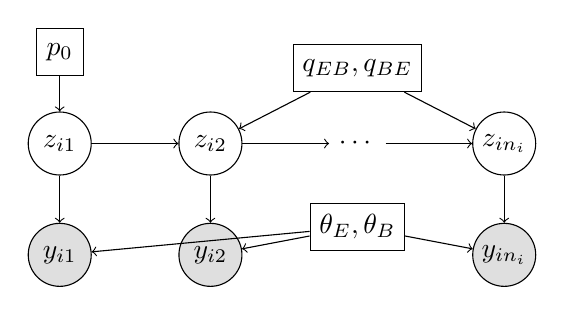
\begin{tikzpicture}[node distance=1.1cm,
  latent/.style={circle, draw, minimum size=8mm, inner sep=1pt},
  obs/.style={circle, draw, fill=gray!25, minimum size=8mm, inner sep=1pt},
  par/.style={rectangle, draw, minimum size=6mm}]
  \node[latent] (z1) {$z_{i1}$};
  \node[latent, right=of z1] (z2) {$z_{i2}$};
  \node[right=of z2] (dots) {$\cdots$};
  \node[latent, right=of dots] (zn) {$z_{in_i}$};
  \node[obs, below=0.6cm of z1] (y1) {$y_{i1}$};
  \node[obs, below=0.6cm of z2] (y2) {$y_{i2}$};
  \node[obs, below=0.6cm of zn] (yn) {$y_{in_i}$};
  \node[par, above=0.45cm of z1] (p0) {$p_0$};
  \node[par, above=0.45cm of dots] (q) {$q_{EB}, q_{BE}$};
  \node[par, below=0.55cm of dots] (th) {$\theta_E, \theta_B$};
  \draw[->] (z1) -- (z2); \draw[->] (z2) -- (dots); \draw[->] (dots) -- (zn);
  \draw[->] (z1) -- (y1); \draw[->] (z2) -- (y2); \draw[->] (zn) -- (yn);
  \draw[->] (p0) -- (z1); \draw[->] (q) -- (z2); \draw[->] (q) -- (zn);
  \draw[->] (th) -- (y1); \draw[->] (th) -- (y2); \draw[->] (th) -- (yn);
\end{tikzpicture}
\caption{Layer~3 as a Bayesian network: observed skips (shaded), hidden moods (white) and unknown parameters (squares). Layer~2 is the same graph with one mood $z_i$ for the whole session.}
\label{fig:network}
\end{figure}

\textbf{Priors.} Layer~1 uses the uniform Beta(1, 1). In Layers~2 and~3, every parameter has a Beta(2, 2) prior, with $\theta_E < \theta_B$. It is weakly informative and keeps the parameters away from 0 and 1, which a mixture could otherwise reach. For the switch probabilities it does not favour long moods, so any stickiness must come from the data. It weighs as much as four observations, against about 63{,}000 pairs of neighbouring tracks. Layers~2 and~3 share these priors, so that any difference between them comes from the switches alone.

\textbf{Assumptions.} Given its mood, a track is skipped independently of the others; the next mood depends only on the current one; all sessions share the same parameters. The last assumption ignores differences between listeners, which we discuss in \cref{sec:discussion}. 

%--------------------------------------------------------------------------
\section{Method}\label{sec:method}
%--------------------------------------------------------------------------

We implemented every algorithm ourselves in Python with NumPy (files \texttt{session\_types.py}, \texttt{mood\_switching.py}, \texttt{posterior.py}). SciPy is used only for random draws and standard densities, pandas for data handling, and Matplotlib for figures.

\textbf{Layer 1.} The Beta prior is conjugate: with $s$ skips in $n$ tracks, $\theta \given \by \sim \text{Beta}(1+s, 1+n-s)$. For $\theta_R - \theta_O$ we use 100{,}000 Monte Carlo draws from each posterior.

\textbf{Likelihood.} All computations are in logs, because a product of hundreds of probabilities underflows. For Layer~3, the \emph{forward algorithm} uses the Markov property to build the sum over all mood sequences one track at a time: with $\alpha_t(j) = P(y_{i1}, \dots, y_{it}, z_{it} = j)$,
\[
\alpha_1(j) = P(z_{i1}=j)\,P(y_{i1}\given j), \qquad
\alpha_t(j) = \Big(\textstyle\sum_k \alpha_{t-1}(k)\, A_{kj}\Big)\, P(y_{it} \given j), \qquad
p(y_i) = \textstyle\sum_j \alpha_{n_i}(j).
\]
After each track we divide the $\alpha_t$ by their sum $c_t$, so they stay between 0 and 1, and $\log p(y_i) = \sum_t \log c_t$.

\textbf{Posterior mode by EM.} The E-step computes, by Bayes' rule, the probability of each type (Layer~2), or of each mood at each track and each pair of moods at neighbouring tracks (Layer~3, with the forward recursion and the same recursion run backwards; this version is known as Baum--Welch). The M-step gives each parameter the mode of a Beta posterior, $(\text{successes} + \alpha - 1)/(\text{trials} + \alpha + \beta - 2)$, with expected counts in place of observed ones. The mode moves when the scale changes: on the log-odds scale used below, the Jacobian $p(1-p)$ turns the Beta(2, 2) prior into the shape of a Beta(3, 3). So we run EM with Beta(3, 3) to find the mode on that scale; the model's prior stays Beta(2, 2). We start EM from 10 random points drawn from the prior, keep the best end point, and check that the log-posterior never decreases. Layer~2 runs 200 iterations. Layer~3 can climb very slowly when the moods look alike, so it stops when an iteration gains less than $10^{-8}$ (at most 2{,}000 iterations).

\textbf{Full posterior by importance sampling.} EM gives a point, not the uncertainty. We use self-normalized importance sampling. We work on the log-odds scale $\phi = \log(p/(1-p))$, so that every draw is a valid set of probabilities, with the prior rewritten using the Jacobian. The proposal is a Student-$t$ with 4 degrees of freedom, centred at the EM mode, with scale $(-H)^{-1}$, where $H$ is the Hessian of the log-posterior at the mode (central differences). Its tails are heavier than the target's, which keeps the weights bounded. Each of the 20{,}000 draws is weighted by posterior/proposal, in logs with log-sum-exp; draws with $\theta_E \ge \theta_B$ get weight 0. We report the ESS, $1/\sum_k \bar w_k^2$, and the largest weight. As a benchmark, a Student-$t$(4) proposal on an exactly Normal target reaches an ESS of 86.6\% in 3 dimensions and 79.9\% in 5. The Monte Carlo error of an estimator is its standard deviation over repeated runs, so we repeat the whole sampling with 10 seeds.

\textbf{Posterior predictive checks.} We draw 1{,}000 parameter sets from the weighted draws (a discrete inverse transform) and simulate sessions with the training lengths. We compare six statistics with the real data: (1)~the \emph{spread} (standard deviation) of skip rates between sessions; (2)~the \emph{gap after a skip}; (3)~the mean \emph{longest run} of skips; (4)~the \emph{gap after shuffling} (20 shuffles); (5)~the \emph{within-session gap}, (2) minus (4); (6)~the number of \emph{skip/play changes} per session. Only switching moods can explain (5) and (6).

\textbf{Additional analysis.} Beyond the model checks, we score how well each layer predicts new listeners: the mean log posterior predictive probability of each test track, given the earlier tracks of its session. A fair coin scores $-0.693$.

%--------------------------------------------------------------------------
\section{Validation on simulated data}\label{sec:validation}
%--------------------------------------------------------------------------

\textbf{The code computes the right likelihood.} It matches values computed by hand, a brute-force sum over all mood sequences for sessions of 1 to 4 tracks (to $2 \times 10^{-16}$), and, with $q_{EB} = q_{BE} = 0$, the Layer~2 log-likelihood (to $4 \times 10^{-12}$).

\textbf{Layer 1.} Over 2{,}000 simulated data sets of 500 tracks, 93.70\% to 94.85\% of the 95\% intervals contain the true rate (0.2, 0.4 or 0.6; Monte Carlo error about 0.5\%).

\textbf{Layers 2 and 3.} We simulated as many sessions as in the training data, with the same lengths, and ran EM and importance sampling. For Layer~2 we used an easy case (types far apart) and a hard case (types close together). Every true value falls inside its 95\% interval (\cref{tab:validation}); in the hard case the intervals are 2 to 4 times wider but still contain the truth. All 10 EM starts reach the same mode in Layer~2. In Layer~3, 8 of 10 do; the other two stay in a flat region where $\theta_E \approx \theta_B \approx 0.41$, with a much lower log-posterior, and are discarded. Comparing proposals (\cref{app:proposals}), the prior gives an ESS of one draw, and a Normal with half the standard deviation only 6\% (Layer~2) and 1.5\% (Layer~3), while the Student-$t$ reaches the benchmark.

\begin{table}[h]
\centering
\small
\caption{Recovery of known values on simulated data: posterior mean and 95\% interval. All true values fall inside their interval.}
\label{tab:validation}
\begin{tabular}{@{}lcccccc@{}}
\toprule
 & \multicolumn{2}{c}{Layer 2, easy} & \multicolumn{2}{c}{Layer 2, hard} & \multicolumn{2}{c}{Layer 3} \\
\cmidrule(lr){2-3}\cmidrule(lr){4-5}\cmidrule(lr){6-7}
 & truth & estimate & truth & estimate & truth & estimate \\
\midrule
$\theta_E$ & 0.05 & 0.050 [0.047, 0.052] & 0.30 & 0.304 [0.295, 0.312] & 0.08 & 0.082 [0.078, 0.086] \\
$\theta_B$ & 0.85 & 0.853 [0.849, 0.857] & 0.55 & 0.554 [0.544, 0.565] & 0.80 & 0.802 [0.795, 0.808] \\
$p_0$      & 0.55 & 0.544 [0.529, 0.559] & 0.55 & 0.568 [0.534, 0.602] & 0.55 & 0.535 [0.517, 0.553] \\
$q_{EB}$   & -- & -- & -- & -- & 0.05 & 0.051 [0.047, 0.054] \\
$q_{BE}$   & -- & -- & -- & -- & 0.06 & 0.063 [0.060, 0.067] \\
\bottomrule
\end{tabular}
\end{table}

%--------------------------------------------------------------------------
\section{Results}\label{sec:results}
%--------------------------------------------------------------------------

\subsection{Diagnostics}

The importance sampling reaches an ESS of 86.3\% for Layer~2 and 79.6\% for Layer~3, close to the benchmarks (86.6\% and 79.9\%). No draw has $\theta_E \ge \theta_B$, so no draw gets weight 0. No single weight dominates: the largest is below 0.0001, at most twice the average $1/20{,}000$. The Monte Carlo error over 10 seeds is about 100 times smaller than the posterior standard deviation (e.g.\ 0.00002 against 0.0023 for $\theta_E$ in Layer~2), so 20{,}000 draws are enough. On Yambda, all 10 EM starts of Layer~2 and 9 of Layer~3 reach the same mode (\cref{app:diagnostics}).

\subsection{Posterior summaries}

\textbf{Layer 1.} The skip rate is 0.4185 [0.4147, 0.4222]. Recommended tracks are skipped less than organic ones (0.392 against 0.445): $\theta_R - \theta_O = -0.054$ [$-0.061$, $-0.046$], and none of the 100{,}000 draws is above zero (\cref{app:layer1}).

\textbf{Layer 2.} About 54\% of sessions are engaged, with 11\% of tracks skipped, and 46\% are browsing, with 76\% skipped (\cref{tab:posterior}). Most sessions are clearly one type: 95\% have $P(\text{Browsing} \given y_i)$ below 0.1 or above 0.9.

\textbf{Layer 3.} The switch probabilities are above zero: $q_{EB} = 0.037$ and $q_{BE} = 0.045$ per track. So an engaged stretch lasts about 27 tracks and a browsing stretch about 22, longer than our longest sessions (20 tracks). So most sessions stay in one mood: a session has 0.59 expected switches on average, and 27\% have at least one expected switch. \Cref{fig:examples} shows how the model reads four real sessions.

\begin{table}[h]
\centering
\small
\caption{Posterior of Layers 2 and 3 on the training data: mean and 95\% interval.}
\label{tab:posterior}
\begin{tabular}{@{}lcc@{}}
\toprule
Parameter & Layer 2 & Layer 3 \\
\midrule
$\theta_E$ & 0.109 [0.105, 0.114] & 0.062 [0.058, 0.067] \\
$\theta_B$ & 0.765 [0.758, 0.771] & 0.853 [0.846, 0.859] \\
$p_0$ & 0.536 [0.520, 0.552] & 0.565 [0.546, 0.583] \\
$q_{EB}$ & -- & 0.0369 [0.0340, 0.0398] \\
$q_{BE}$ & -- & 0.0454 [0.0419, 0.0490] \\
Mean Engaged stretch $1/q_{EB}$ (tracks) & -- & 27.2 [25.1, 29.4] \\
Mean Browsing stretch $1/q_{BE}$ (tracks) & -- & 22.1 [20.4, 23.9] \\
Long-run share of Browsing tracks & -- & 0.448 [0.427, 0.470] \\
\bottomrule
\end{tabular}
\end{table}

\begin{figure}[h]
  \centering
  \includegraphics[width=0.6\linewidth]{figures/layer3_example_sessions.pdf}
  \caption{Layer~3: posterior probability of Browsing along four training sessions (dots: skips up, plays down). The model detects a switch after a run of skips or plays, and reads an isolated play inside a browsing stretch as a play, not as a switch.}
  \label{fig:examples}
\end{figure}

\subsection{Model checking}

\Cref{tab:checks} compares the three layers. Layer~1 fails every check: tracks are not independent. Layer~2 gets close on the differences between sessions (spread 0.341 against 0.358), but its tracks are independent given the type, so the order cannot matter: the within-session gap is 0 (real 0.101), and sessions change from skip to play too often (3.95 against 2.74). Layer~3 is closer on every statistic about runs: 2.94 changes per session and a longest run of 4.37. It also reproduces the sessions with a middle skip rate (\cref{fig:rates}, \cref{app:diagnostics}): 27.6\% of simulated sessions have 30\% to 70\% skips, against 26.7\% in the real data and 16.1\% for Layer~2.

But Layer~3 overshoots: its within-session gap is 0.178 against 0.101, and its gap after shuffling falls to 0.406 (real 0.512). Sessions with no skip are still too rare (13.2\% against 22.1\%), and every statistic still rejects every layer.

\begin{table}[h]
\centering
\small
\caption{Posterior predictive checks: real value and mean over 1{,}000 simulated data sets. For every statistic and every layer, the real value lies outside the central 95\% of the simulations.}
\label{tab:checks}
\begin{tabular}{@{}lcccc@{}}
\toprule
Statistic & Real & Layer 1 & Layer 2 & Layer 3 \\
\midrule
Spread of skip rates & 0.358 & 0.129 & 0.341 & 0.332 \\
Gap after a skip & 0.613 & 0.000 & 0.441 & 0.583 \\
Longest run of skips & 4.77 & 2.73 & 3.60 & 4.37 \\
Gap after shuffling & 0.512 & 0.000 & 0.441 & 0.406 \\
Within-session gap & 0.101 & 0.000 & 0.000 & 0.178 \\
Skip/play changes & 2.74 & 7.09 & 3.95 & 2.94 \\
\bottomrule
\end{tabular}
\end{table}



\subsection{Sensitivity and additional analysis}

With Beta(1, 1) or Beta(5, 5) on every parameter, the posterior means and intervals of Layers~2 and~3 agree to the third decimal (\cref{app:sensitivity}). The largest change is for $q_{BE}$, from 0.0453 to 0.0456, far below its posterior standard deviation (0.0018). On new listeners, Layer~1 scores $-0.678$, Layer~2 $-0.479$ and Layer~3 $-0.446$ (fair coin: $-0.693$).

%--------------------------------------------------------------------------
\section{Discussion and conclusion}\label{sec:discussion}
%--------------------------------------------------------------------------

Our main conclusion is that: yes, a hidden mood can be inferred from skips alone. Each layer answered a question raised by the previous one. Layer~1 showed that skips come in runs: a gap after a skip of 0.613, where independent tracks would give 0. The shuffle test split this gap in two: 0.512 comes from differences between sessions, and 0.101 from the order of the tracks. Layer~2 captures most of the first part (0.441) and none of the second; Layer~3 captures both. Listening falls into two regimes: in one, about 6\% of tracks are skipped; in the other, about 85\%. We call them moods, but the model only sees skips: the hidden state could also be an activity (background listening or active search), a playlist or a device. Earlier work found four session types by clustering \citep{meggetto2021skipping}; our two moods are a simpler summary, but they come with their uncertainty, and they separate differences between sessions from the order of the tracks.

Moods can change in a session, but rarely: a mood lasts 22 to 27 tracks on average and a session has 0.59 expected switches. So a session's first tracks say a lot about the rest of it: a service could notice browsing after a few skips and adapt what it suggests. Prediction shows this gain: on new listeners, Layer~3 scores $-0.446$, against $-0.678$ for Layer~1 and $-0.693$ for a fair coin. Browsing also ends a little sooner than engaged listening: $q_{BE}$ is above $q_{EB}$, and their intervals do not overlap. Finally, recommended tracks are skipped less than tracks the listener found alone (0.392 against 0.445). One possible reason is that listeners who choose their own tracks are more often searching, although our data cannot tell the cause.

The scores of our models on the checks do not only reject our models, but show in which direction lies the truth. The within-session gap is 0 for Layer~2, 0.178 for Layer~3 and 0.101 in the real data. Layer~2 has too little order effect and Layer~3 too much: Layer~3 explains part of the differences between sessions by switches inside sessions. So part of what it calls switches is probably differences between listeners: some people skip much more, or much less, than either mood allows. 

Our study is limited in some parts. First, the model isn't complete: every layer fails its predictive checks, so the real uncertainty is larger than our intervals. Second, our data choices matter. We cut sessions at 20 tracks before the analysis, for computing reasons, but our analysis revealed that a mood lasts 22 to 27 tracks. Thus, few sessions have time to switch behaviour, and the switch probabilities rest on few examples. \Cref{fig:position} shows no effect of the position within 20 tracks, but only on average: opposite patterns can cancel out. Besides,  a pattern such as browsing first and then settling would mostly fall after the cut. 
The results also depend on our other definitions (50\% threshold, 60~s of silence, timestamp reading), and a binary skip mixes early and late skips \citep{montecchio2020skipping}.
Third, we left out who listens and what is played. We kept one session per user and context for independent draws. So we learn little about each listener, and we ignore the listener's history, the music style, and whether a track is already known or liked. All of this is now hidden inside the mood. It may also explain the context effect, which can reflect different tracks and habits rather than the context itself.

Each limitation suggests a next step. Give each listener their own tendency to skip, on top of the moods, to separate listeners from moods. Use longer sessions, to see more switches and test whether browsing sessions settle. Add what is known about listeners and tracks: the data set also records likes, dislikes and audio embeddings of the tracks \citep{yandex2025card}. Fit Layers~2 and~3 per context, try three moods, and cross-check the posterior with Metropolis--Hastings.

%--------------------------------------------------------------------------
%  References (not counted in the 8 pages)
%--------------------------------------------------------------------------

\clearpage   % the references start on a new page

\bibliographystyle{apalike}
\bibliography{references}

%--------------------------------------------------------------------------
%  Appendices (optional, not counted in the 8 pages)
%--------------------------------------------------------------------------
% Title page of the appendices
\clearpage
\thispagestyle{fancy}
\begin{center}
\vspace*{\fill}
{\LARGE\sc Appendices}

\bigskip
{\large Supplementary material, not counted in the 8 pages}

\vspace{1.5cm}
\begin{tabular}{@{}ll@{}}
A & Layer 1: position, context and predictive checks \\[4pt]
B & Choice of the importance sampling proposal \\[4pt]
C & Sensitivity to the prior \\[4pt]
D & Diagnostics and additional checks \\[4pt]
E & Code: which file produces what \\
\end{tabular}
\vspace*{\fill}
\end{center}
\clearpage

\appendix
\crefalias{section}{appendix}

\section{Layer 1: position, context and predictive checks}\label{app:layer1}

\begin{figure}[H]
  \centering
  \includegraphics[width=0.46\linewidth]{figures/layer1_skip_rate_by_position.pdf}
  \caption{Share of tracks skipped at each position in the session, for each context (all users). It is almost the same at every position, which supports our assumption that the skip probability does not depend on the position.}
  \label{fig:position}
\end{figure}

\begin{figure}[H]
  \centering
  \includegraphics[width=0.48\linewidth]{figures/layer1_posterior_by_context.pdf}
  \caption{Layer~1: posterior of the skip rate in each context, from 100{,}000 draws (training users).}
\end{figure}

\begin{table}[H]
\centering
\small
\caption{Layer~1 posterior predictive checks, from 1{,}000 simulated data sets.}
\begin{tabular}{@{}lccc@{}}
\toprule
Statistic & Real data & Simulated mean & Simulated 95\% range \\
\midrule
Spread of skip rates & 0.3584 & 0.1294 & 0.1268 to 0.1323 \\
Gap after a skip & 0.6134 & $-0.0001$ & $-0.0077$ to 0.0078 \\
Longest run of skips & 4.7731 & 2.7329 & 2.6864 to 2.7796 \\
\bottomrule
\end{tabular}
\end{table}

The posterior mean of $\theta$ stays between 0.41843 and 0.41852 under the priors Beta(1, 1), Beta(2, 8), Beta(8, 2) and Beta(40, 60).

\section{Choice of the importance sampling proposal}\label{app:proposals}

\begin{table}[H]
\centering
\small
\caption{Three proposals on the simulated data, 20{,}000 draws each. The prior spreads its draws over the whole space while the posterior is tiny, so one draw takes all the weight. The Normal with half the standard deviation is centred correctly, but its lighter tails make the weights unequal.}
\label{tab:proposals}
\begin{tabular}{@{}lcccc@{}}
\toprule
 & \multicolumn{2}{c}{Layer 2} & \multicolumn{2}{c}{Layer 3} \\
\cmidrule(lr){2-3}\cmidrule(lr){4-5}
Proposal & ESS share & largest weight & ESS share & largest weight \\
\midrule
Student-$t$ (4 df) at the mode & 86.9\% & 0.0001 & 80.0\% & 0.0001 \\
Prior Beta(2, 2) & 1 draw & 1 & 1 draw & 1 \\
Normal at the mode, half the sd & 6.2\% & 0.008 & 1.5\% & 0.033 \\
\bottomrule
\end{tabular}
\end{table}

\section{Sensitivity to the prior}\label{app:sensitivity}

\begin{table}[H]
\centering
\small
\caption{Posterior means under three priors, applied to every parameter.}
\begin{tabular}{@{}llccc@{}}
\toprule
Layer & Parameter & Beta(1, 1) & Beta(2, 2), main & Beta(5, 5) \\
\midrule
2 & $\theta_E$ & 0.10911 & 0.10916 & 0.10928 \\
2 & $\theta_B$ & 0.76461 & 0.76460 & 0.76462 \\
2 & $p_0$      & 0.53552 & 0.53545 & 0.53557 \\
\midrule
3 & $\theta_E$ & 0.06239 & 0.06235 & 0.06244 \\
3 & $\theta_B$ & 0.85257 & 0.85259 & 0.85266 \\
3 & $p_0$      & 0.56472 & 0.56461 & 0.56464 \\
3 & $q_{EB}$   & 0.03678 & 0.03687 & 0.03703 \\
3 & $q_{BE}$   & 0.04530 & 0.04539 & 0.04559 \\
\bottomrule
\end{tabular}
\end{table}

\section{Diagnostics and additional checks}\label{app:diagnostics}

\begin{figure}[H]
  \centering
  \includegraphics[width=0.42\linewidth]{figures/layer3_skip_rate_per_session.pdf}
  \caption{Skip rate per session: real training sessions against sessions simulated from Layer~3 (20 posterior draws). Layer~3 fills the middle but gives too few sessions with no skip or only skips.}
  \label{fig:rates}
\end{figure}

\begin{figure}[H]
  \centering
  \includegraphics[width=0.48\linewidth]{figures/layer2_em_convergence.pdf}\hfill
  \includegraphics[width=0.48\linewidth]{figures/layer3_em_convergence.pdf}
  \caption{EM convergence: distance to the final log-posterior along the iterations, for the 10 starts of Layer~2 (left) and Layer~3 (right). In grey, the Layer~3 start that stays in the flat region where $\theta_E \approx \theta_B$.}
\end{figure}

\begin{figure}[H]
  \centering
  \includegraphics[width=0.7\linewidth]{figures/layer2_posterior.pdf}\\
  \includegraphics[width=\linewidth]{figures/layer3_posterior.pdf}
  \caption{Marginal posteriors of Layer~2 (top) and Layer~3 (bottom), as weighted histograms of the importance sampling draws. They are narrow and close to Normal, as the ESS suggests.}
\end{figure}

\begin{figure}[H]
  \centering
  \includegraphics[width=0.48\linewidth]{figures/layer2_predictive_checks.pdf}\hfill
  \includegraphics[width=0.48\linewidth]{figures/layer3_predictive_checks.pdf}
  \caption{Posterior predictive checks of Layer~2 (left) and Layer~3 (right): 1{,}000 simulated data sets (histograms) and the real value (line) for the six statistics.}
\end{figure}

\begin{figure}[H]
  \centering
  \includegraphics[width=0.5\linewidth]{figures/layer2_skip_rate_per_session.pdf}
  \caption{Skip rate per session: real training sessions against sessions simulated from Layer~2.}
\end{figure}

\section{Code: which file produces what}\label{app:code}

Every number, table and figure comes from the code in \texttt{code/}, run with \texttt{bash run\_all.sh} (about 25 minutes; seed 2026).
\begin{itemize}
  \item \texttt{prepare\_yambda.py}: builds \texttt{data/sessions.csv} from Yambda (\cref{sec:data}).
  \item \texttt{layer1\_baseline.ipynb}: \cref{fig:position}, Layer~1 results, \cref{app:layer1}.
  \item \texttt{layer2\_session\_types.ipynb}: Layer~2 columns of \cref{tab:validation,tab:posterior,tab:checks}, \cref{tab:proposals}, Layer~2 figures of \cref{app:diagnostics}.
  \item \texttt{layer3\_mood\_switching.ipynb}: Layer~3 columns of the same tables, \cref{fig:examples,fig:rates}, Layer~3 figures of \cref{app:diagnostics}.
  \item Shared functions: \texttt{checks.py} (statistics), \texttt{posterior.py} (EM driver, importance sampling, predictive checks), \texttt{session\_types.py} (Layer~2), \texttt{mood\_switching.py} (Layer~3).
\end{itemize}

\end{document}
